\documentclass{beamer}
\usetheme{Warsaw}

\usepackage[utf8]{inputenc}
\usepackage{fancybox}
\usepackage{multimedia} 
\usepackage{subfig}
\usepackage{amsmath}
\usepackage{hyperref}
\usepackage[all]{xy}
\usepackage{algorithm}
%\usepackage{arevmath}     % For math symbols
\usepackage[noend]{algpseudocode}

\begin{document}


\title[Angewandte Mathematik] % (optional, only for long titles)
{Angewandte Mathematik
\\
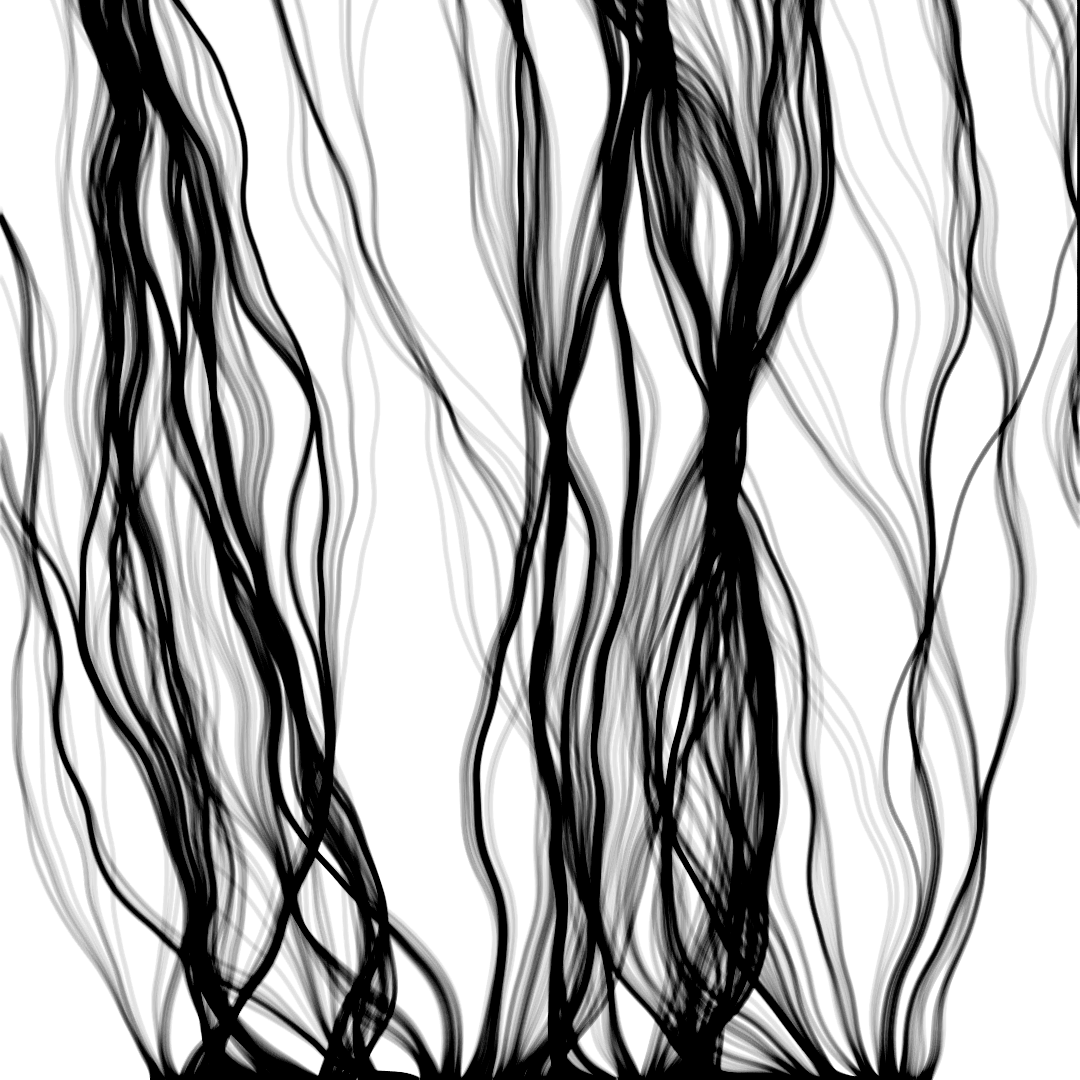
\includegraphics[scale=0.15]{images/cover}
}
\subtitle{}
\author[Dr. Johannes Riesterer] % (optional, for multiple authors)
{Dr.  rer. nat. Johannes Riesterer}

\date[KPT 2004] % (optional)
{}

\subject{Angewandte Mathematik}



\frame{\titlepage}



\begin{frame}
    \frametitle{Angewandte Mathematik}
\framesubtitle{Lebesgue Integral}
    \begin{block}{Indikatorfunktion}
Für eine Teilmenge $A \subset \mathbb{R}^n$ heißt
$$ 1_A (x): = \begin{cases} 1 \text{  falls }   x \in A  \\  0  \text{  sonst}  \end{cases}$$
Indikatorfunktion.
\end{block}

\begin{figure}[H]
      \centering
    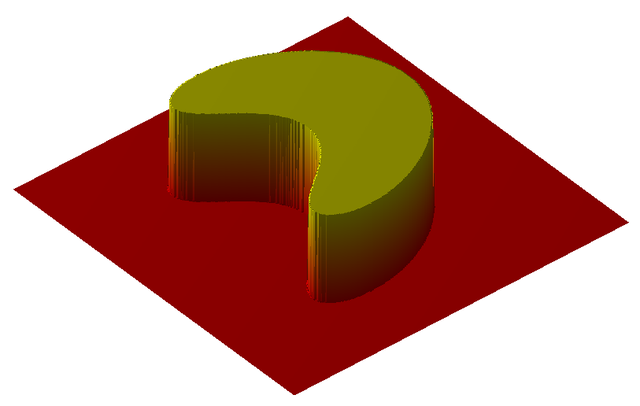
\includegraphics[width=0.6\textwidth]{images/640px-Indicator_function_illustration}
      \caption{Quelle: Wikipedia: https://commons.wikimedia.org/wiki/File:Indicator\_function\_illustration.png}

\end{figure}

 \end{frame}


\begin{frame}
    \frametitle{Angewandte Mathematik}
\framesubtitle{Lebesgue Integral}
    \begin{block}{Sinnvoller Integralbegriff}
Definiere Integral über Funktionen so, dass $\int 1_A d \mu = \mu(A)$
\end{block}

 \end{frame}

\begin{frame}
    \frametitle{Angewandte Mathematik}
\framesubtitle{Lebesgue Integral}
    \begin{block}{Treppenfunktion}
Eine Funktion 
$$ \varphi(x) := \sum_{k=1}^m c_k 1_{I_k}(x)$$ mit $c_k \in \mathbb{R}$ und $I_k \in \mathbb{I}(n)$ mit $I_i \cap I_h = \emptyset$ für $i \neq j$
heißt Treppenfunktion.
\end{block}


\begin{figure}[H]
      \centering
    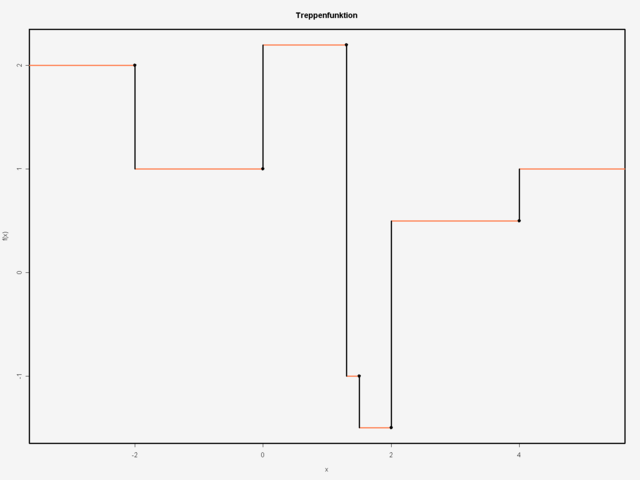
\includegraphics[width=0.4\textwidth]{images/640px-Stepfunction1}
      \caption{Quelle: Wikipedia: https://commons.wikimedia.org/wiki/File:Stepfunction1.png}

\end{figure}
 \end{frame}


\begin{frame}
    \frametitle{Angewandte Mathematik}
\framesubtitle{Lebesgue Integral}
    \begin{block}{Vektorraum der Indikatorfunktionen}

Seien $\varphi(x) =   \sum_{k=1}^m  c_k 1_{I_k}$ und $\psi(x) =  \sum_{j=1}^l  u_j 1_{I_j}$. Dann definiert
$(\varphi + \psi)(x) := \sum_{k=1}^m \sum_{j=1}^l   (c_k + u_j) 1_{I_{k,j}}$ mit $I_{k,j}:= I_k \cap I_j$ eine Treppenfunktion (nach entsprechender Umnummerierung zu einem einzigen Summenzeichen).
\end{block}

 \end{frame}


\begin{frame}
    \frametitle{Angewandte Mathematik}
\framesubtitle{Lebesgue Integral}
    \begin{block}{Integral von Treppenfunktionen}
Für eine Treppenfunktion $ \varphi(x) := \sum_{k=1}^m c_k 1_{I_k}$ definieren wir das Integral durch
$$\int_{\mathbb{R}^n} \varphi d\mu := \sum_{k =1}^m  c_k \mu(I_k) \; . $$
\end{block} 
\end{frame}


\begin{frame}
    \frametitle{Angewandte Mathematik}
\framesubtitle{Lebesgue Integral}
    \begin{block}{Eigenschaften des Integrals von Treppenfunktionen}
Seien $\varphi(x) =   \sum_{k=1}^m  c_k 1_{I_k}$ und $\psi(x) =  \sum_{j=1}^l  u_j 1_{I_j}$ zwei Treppenfunktionen.
Für das Integral von Treppenfunktionen gilt:
\begin{itemize}
\item Ist $\varphi(x) = \psi(x)$ für alle $x$, dann ist $\int_{\mathbb{R}^n} \varphi d\mu = \int_{\mathbb{R}^n} \psi d\mu$ (Das Integral hängt nicht von der Zerlegung der Treppenfunktion ab und  ist wohldefiniert)
\item $\int_{\mathbb{R}^n} \alpha \varphi  + \beta \psi d\mu = \alpha \int_{\mathbb{R}^n}  \varphi d\mu + \beta  \int_{\mathbb{R}^n}  \psi d\mu$
\item $ \biggl|  \int_{\mathbb{R}^n} \varphi d\mu  \biggr| \leq \int_{\mathbb{R}^n} | \varphi | d\mu$
\item Ist $\varphi(x) \leq \psi(x)$ für alle $x$, so ist $\int_{\mathbb{R}^n} \varphi d\mu \leq \int_{\mathbb{R}^n} \psi d\mu$ 
\end{itemize}
\end{block}

 \end{frame}


\begin{frame}
    \frametitle{Angewandte Mathematik}
\framesubtitle{Beweis}

Der Beweis wird über eine vollständige Induktion geführt. Der Induktionsanfang ist einfach zu zeigen. 
Wir nehmen an, die Aussage gilt für alle Dimensionen $k < n$.
Zerlege $\mathbb{R}^n = \mathbb{R}^p \times \mathbb{R}^{n-p}$. Jeder Quader $I \in \mathbb{I}(n)$ zerlegt sich damit ebenfalls in ein Produkt 
$I = I' \times I''$ mit $I'  \in \mathbb{I}(p)$ und  $I''  \in \mathbb{I}(n-p)$ und für $z = (x,y) \in  \mathbb{R}^p \times \mathbb{R}^{n-p}$ gilt $1_{I} (z) = 1_{I'}(x) \cdot 1_{I''}(y)$. Es sei nun $\varphi(z):=   \sum_{k=1}^m  c_k 1_{I_k}(z)$ eine Treppenfunktion auf $ \mathbb{R}^p \times \mathbb{R}^{n-p}$. Für jedes $y \in \mathbb{R}^{n-p}$ definiert  $\varphi_y(x)=   \sum_{k=1}^m  c_k 1_{I''_k}(y) \cdot 1_{I'_k}(x)$ eine Treppenfunktion auf $\mathbb{R}^{p}$. 
Nach Induktionsvoraussetzung hängt das Integral 
$$\int_{\mathbb{R}^p}  \varphi_y(x) d \mu' = \sum_{k=1}^m  c_k \mu'(I'_k)  \cdot 1_{I''_k}(y)  =: \phi(y)$$
nicht von der Zerlegung der Treppenfunktion ab.  \end{frame}

\begin{frame}
    \frametitle{Angewandte Mathematik}
\framesubtitle{Beweis}

$\phi(y)$ ist wiederum eine Treppenfunktion auf $\mathbb{R}^{n-p}$ und nach Induktionsvoraussetzung hängt das Integral 
$$\int_{\mathbb{R}^{n-p}}  \phi(y) d \mu'' = \sum_{k=1}^m  c_k \mu'(I'_k)  \cdot \mu'' (I''_k)(y) $$
nicht von der Zerlegung der Treppenfunktion ab. Somit gilt
\begin{align*}
\int_{\mathbb{R}^{n-p}} \int_{\mathbb{R}^p}  \varphi_y(x) d \mu'  d \mu''  & =   \sum_{k=1}^m  c_k \mu'(I'_k)  \cdot \mu''(I''_k)(y) \\
& = \sum_{k=1}^m  c_k  \mu(I_k)  = \int_{\mathbb{R}^n} \varphi(z) d\mu\;.
\end{align*}
Die linke Seite hängt  damit nicht von der Zerlegung der Treppenfunktion ab und alle Behauptungen können so auf den Fall $n=1$ zurückgeführt werden.
 \end{frame}


\begin{frame}
    \frametitle{Angewandte Mathematik}
\framesubtitle{Lebesgue Integral}
    \begin{block}{Satz von Fubini für Treppenfunktionen}
Es gilt $$\int_{\mathbb{R}^n} \varphi(x,y) d \mu = \int_{\mathbb{R}^{n-p}} \biggl (\int_{\mathbb{R}^{p}}  \varphi(x,y) d \mu' \biggr ) d \mu''$$
\end{block}
    \begin{block}{Beweis}
Folgt direkt aus Beweis des letzten Satzes.
\end{block}
 \end{frame}


\begin{frame}
    \frametitle{Angewandte Mathematik}
\framesubtitle{Lebesgue Integral}
    \begin{block}{Hüllreihe}
Eine Hüllreihe zu einer Funktion $f :\mathbb{R}^n \to \mathbb{R}$ ist eine Reihe $\phi(x):= \sum_{k=1}^{\infty} c_k  1_{I_k} (x)$ mit den folgenden Eigenschaften:
\begin{itemize}
\item $c_k \in \mathbb{R}$ sind positive reelle Zahlen $c_k >0$.
\item $I_k \subset \mathbb{R}^n$ sind offene Quader.
\item Für alle $x \in \mathbb{R}^n$ gilt $|f(x) | \leq \phi(x)$.
\end{itemize}
\end{block}

 \begin{block}{Inhalt einer Hüllreihe}
Der Inhalt einer Hüllreihe $\phi(x):= \sum_{k=1}^{\infty} c_k  1_{I_k} (x)$ ist definiert durch 
$$I (\phi) := \sum_{k=1}^{\infty} c_k \;  \mu(I_k) \; .$$
\end{block}

 \end{frame}


\begin{frame}
    \frametitle{Angewandte Mathematik}
\framesubtitle{Lebesgue Integral}
    \begin{block}{ $L^1$-Halbnorm }
Die $L^1$-Halbnorm einer Funktion $f :\mathbb{R}^n \to \mathbb{R}$ ist definiert durch das Infimum der Inhalte der Hüllreihen zu $f$
$$ || f ||_1 : = \inf  \biggl \{   I(\phi) \; | \; \phi  \text{ ist Hüllreihe zu  }  f \biggr \} \; .$$
\end{block}

 \end{frame}






\begin{frame}
    \frametitle{Angewandte Mathematik}
\framesubtitle{Lebesgue Integral}
    \begin{block}{Rechenregeln für Hüllfunktionen}
Für $f,g : \mathbb{R}^n \to \mathbb{R}$ und $c \in \mathbb{R}$ gilt:
 \begin{itemize}
\item $|| cf ||_1 \leq |c| || f ||_1$. 
\item $|| f +g ||_1 \leq  ||f ||_1 + ||g||_1$
\item Aus $f (x) \leq g(x)$ für alle $x$ folgt $|| f ||_1 \leq || g ||_1$.
\end{itemize}

\end{block}
 \end{frame}


\begin{frame}
    \frametitle{Angewandte Mathematik}
\framesubtitle{Beweis}
 \begin{itemize}
\item Für eine Hüllreihe $\varphi$ von $f$ ist $|c| \cdot \varphi$ eine Hüllreihe von $c \cdot f$. 
\item Da $|f +g | \leq | f | + | g |$ folgt Behauptung aus (iii) und der verallgemeinerten Dreiecksungleichung.
\item Hüllreihen sind immer größer-gleich der Funktion und damit haben größere Funktionen größere Hüllreihen.
\end{itemize}
 \end{frame}



\begin{frame}
    \frametitle{Angewandte Mathematik}
\framesubtitle{Lebesgue Integral}
    \begin{block}{Verallgemeinerte Dreiecksungleichung}
Für nicht negative Funktionen $f_k  :\mathbb{R}^n \to \mathbb{R}_{\geq 0}$ gilt
$$ \biggl | \biggl | \sum_{k=1}^{\infty} f_k \biggr | \biggr |_1 \leq  \sum_{k=1}^{\infty} || f_k  ||_1 \; .$$
\end{block}

 \end{frame}



\begin{frame}
    \frametitle{Angewandte Mathematik}
\framesubtitle{Beweis}
$ 1 \cdot 1_I$ ist eine Hüllreihe von $1_i$ und damit gilt $|| 1_I || \leq \mu(I)$. 
Sei $\phi(x) = \sum_k c_k 1_{I_k} $ eine Hüllreihe von $1_i$ und $\epsilon >0$. Da $\phi(x) \geq 1$ gibt es für jedes $x$ einen Index $N(x)$ mit 
$\sum_{k=1}^{N(x)} c_k 1_{I_k} \geq 1 - \epsilon$. Da die $I_k$ offen sind, gibt es für jedes $x$ eine Umgebung $U(x)$, so dass letztere Gleichung gilt. Da $\bar{I}$ kompakt ist (beschränkt und abgeschlossen), überdecken endlich viele $U(x_1), \cdots , U(x_n)$ den Quader $I$. Mit $N:= \max \{ N(x_1), \cdots , N(x_n)$ folgt $\sum_{k=1}^N c_k 1_{I_k} \geq (1-\epsilon) 1_I$. Aus den Rechenregeln für Treppenfunktionen (iii) folgt
$$ I (\phi) = \sum_k c_k \mu(I_k) \geq \sum_{k=1}^N c_k \mu (I_k) \geq (1 - \epsilon) \mu(I) \;.$$
Mit $\epsilon \to 0$ folgt $I (\phi) \geq \mu(i)$ und damit insgesamt die Behauptung.  
 \end{frame}


\begin{frame}
    \frametitle{Angewandte Mathematik}
\framesubtitle{Lebesgue Integral}
    \begin{block}{Norm und Integral}
Für jede Treppenfunktion $\varphi$ auf $\mathbb{R}^n$ gilt
$$ || \varphi ||_1 = \int | \varphi | d \mu  \; .$$
\end{block}

 \end{frame}




\begin{frame}
    \frametitle{Angewandte Mathematik}
\framesubtitle{Lebesgue Integral}
    \begin{block}{Integrierbare Funktionen}
Eine Funktion $f : \mathbb{R}^n \to \mathbb{R}$ heißt integrierbar, falls eine Folge von Treppenfunktionen  $\varphi_k$ existiert mit
$$ || f -  \varphi_k ||_1 \to 0 \text{ für } k \to \infty \;. $$
\end{block}

    \begin{block}{Integrierbare Funktionen}
\begin{itemize}
\item Die reelle Zahlenfolge $\int \varphi_k d\mu$ ist eine Cauchyfolge und damit konvergent. 
\item Der Grenzwert ist unabhängig von der Folge $\varphi_k$.
\end{itemize}
\end{block}


 \end{frame}



\begin{frame}
    \frametitle{Angewandte Mathematik}
\framesubtitle{Beweis}
Für Treppenfunktionen $\psi$ und $\xi$ gilt 
\begin{align*}
\biggl | \int \psi d \mu - \int \xi d \mu \biggr |  &  \leq \int | \psi - \xi | d \mu = || \psi - \xi ||_1 \\
& \leq  || \psi - f ||_1 +  || f - \xi ||_1
\end{align*}
woraus die Behauptungen folgen.
 \end{frame}


\begin{frame}
    \frametitle{Angewandte Mathematik}
\framesubtitle{Lebesgue Integral}
    \begin{block}{Integral und Norm}
Ist $f$ über $\mathbb{R}^n$ integrierbar, so auch $|f|$ und es gilt
$$ \biggl | \int f d \mu \biggr | \leq \int  | f | d \mu = || f ||_1 \; .$$
\end{block}

 \end{frame}


\begin{frame}
    \frametitle{Angewandte Mathematik}
\framesubtitle{Beweis}
Sei $f$ integrierbar und $\varphi_k$ eine Folge von Treppenfunktionen mit $|| f - \varphi_k ||_1 \to 0$. 
Aus $\bigl | | f | - | \varphi_k | \bigr | \leq | f -\varphi | $ ergibt sich wegen der Monotonie der $L^1$-Norm
$$\bigl |  \bigl |  | f | - | \varphi_k | \bigr | \bigr |_1 \leq \bigl |  \bigl |   f  -  \varphi_k  \bigr | \bigr |_1  \; .$$ 
Damit gilt $\bigl |  \bigl |  | f | - | \varphi_k | \bigr | \bigr |_1 \to 0$ und somit ist $|f|$ integrierbar und mit der Abschätzung von Beträgen für Treppenfunktionen gilt 
\begin{align*}
\biggl | \int f d \mu \biggr | = \biggl | \lim_k \int \varphi_k d \mu \biggr | \leq  \int |\varphi_k| d \mu = \int |f| d\mu
\end{align*} 
und damit der erste Teil der Behauptung. 
Mit der Dreiecksungleichung erhalten wir
$$ || f || - ||  f - \varphi ||_1 \leq || \varphi_k ||_1  \leq || f ||_1 + || f - \varphi_k ||_1 $$
und wegen $|| \varphi_k ||_1 = \int | \varphi_k | d \mu \to \int | f | d \mu$ folgt die Behauptung.
 \end{frame}


\begin{frame}
    \frametitle{Angewandte Mathematik}
\framesubtitle{Lebesgue Integral}
    \begin{block}{Rechenregeln}
Sind $f$ und $g$ integrierbar, so gilt
\begin{itemize}
\item $ \alpha f + \beta g$ mit $\alpha, \beta \in \mathbb{R}$ ist integrierbar mit 
$$\int \alpha f + \beta g d\mu = \alpha \int f d\mu + \beta \int g d \mu \; .$$ 
\item Aus $f(x) \leq g(x)$ für alle $x \in \mathbb{R}^n$ folgt $\int f d \mu \leq \int g d \mu$.
\item Ist $g$ zusätzlich beschränkt, so ist auch $f \cdot g$ integrierbar.
\end{itemize}

\end{block}

 \end{frame}


\begin{frame}
    \frametitle{Angewandte Mathematik}
\framesubtitle{Beweis}
\begin{itemize}
\item Sind $\phi_k$ und $\psi_k$ approximierende Folge von  Treppenfunktionen von $f$ und $g$, so ist $\alpha \phi_k + \beta \psi_k$ eine approximierende Folge von $\alpha f + \beta g$.
\item Es  ist $\int (g-f) d \mu = || g - f ||_1 \geq 0$.
\end{itemize}
 \end{frame}




\begin{frame}
    \frametitle{Angewandte Mathematik}
\framesubtitle{Lebesgue Integral}
    \begin{block}{Min Max}
Ist $f$ integrierbar, so auch $f^+ := \max(f,0)$ und $f^- := \min(f,0)$. Damit ist $f = f^+ + f^-$ genau dann integrierbar, wenn $f^+$ und $f^-$ integrierbar sind. Da $- f^- \geq 0$ ist, kann man sich in Beweisen häufig auf den Fall $f \geq 0$ beschränken.
\end{block}
    \begin{block}{Beweis}
Es ist $ \max(f,0) = \frac{1}{2} (f + | f |)$ und  $ \min(f,0) = \frac{1}{2} (f - | f |)$ und die Behauptung folgt aus den Rechenregeln.

\end{block}
 \end{frame}


\begin{frame}
    \frametitle{Angewandte Mathematik}
\framesubtitle{Lebesgue Integral}
    \begin{block}{Integration über Teilmengen}
Für  eine Teilmenge $A \subset \mathbb{R}^n$ und eine Funktion $f: A \to \mathbb{R}$ heißt
$$  f_A (x) : = \begin{cases}  f(x) \text{ für } x \in A \\ 0  \text{ für } x \in \mathbb{R}^n \setminus A \end{cases}$$ 
die triviale Fortsetzung von $f$ auf $\mathbb{R}^n$. $f$ heißt integrierbar über $A$, falls $f_A$ über $\mathbb{R}^n$ integrierbar ist und in diesem Fall bezeichnen wir mit $$ \int_A f(x) d \mu := \int f_A (x) d\mu$$ als das Integral von $f$ über $A$.
\end{block}

 \end{frame}



\begin{frame}
    \frametitle{Angewandte Mathematik}
\framesubtitle{Lebesgue Integral}
    \begin{block}{Kleiner Satz von B. Levi}
Zu $f: \mathbb{R}^n \to \mathbb{R}$ gebe es eine monoton wachsende Folge $\varphi_k$ von Treppenfunktionen mit
\begin{itemize}
\item Für alles $x \in \mathbb{R}^n$ git $\lim_{k \to \infty} \varphi(x) =  f(x)$. $f$ ist also die punktweise gebildete Grenzfunktion der $\varphi_k$.
\item Die reelle Folge der Integrale $\int \varphi_k d \mu $ ist beschränkt.
\end{itemize}
Dann ist $f$ integrierbar und es gilt $$ \int f d \mu = lim_{k \to \infty}  \int \varphi_k d \mu \; .$$
\end{block}

 \end{frame}




\begin{frame}
    \frametitle{Angewandte Mathematik}
\framesubtitle{Beweis}
Aus $f  - \varphi_k = \sum_{i=k}^{\infty} (\varphi_{k+1} - \varphi_k)$ folgt mit der verallgemeinerten Dreiecksungleichung  und dem Satz über Norm und Integration 
\begin{align*}
|| f - \varphi_k ||_1 \leq \sum_{i=k}^{\infty} \int | \varphi_{i+1} - \varphi_i | d \mu =  \sum_{i=k}^{\infty} \biggl ( \int  \varphi_{i+1}d \mu -  \int \varphi_i  d \mu \biggr ) \; .
\end{align*}
Die Folge $\int \varphi_k$ ist monoton wachsend und beschränkt und damit konvergent. Bezeichnen wir mit $I$ den Grenzwert, so folgt 
$|| f -\varphi_k ||_1 \leq I - \int \varphi_k d \mu $. Also gilt $|| f -\varphi_k ||_1 \to 0$ für $k \to \infty$ und damit ist $f$ integrierbar und mit der Definition des Integrals folgt die Behauptung.
 \end{frame}



\begin{frame}
    \frametitle{Angewandte Mathematik}
\framesubtitle{Lebesgue Integral}
    \begin{block}{Offene Mengen}
Eine Menge $U \subset \mathbb{R}^n$ heißt offen, falls für alle $a \in U$ ein Radius $r >0$ existiert, so dass der Ball $B_r(a) : = \{ x \in \mathbb{R}^n \; | \; ||x -a|| \leq r \} \subset U$ in $U$ enthalten ist.
\end{block}

 \end{frame}

\begin{frame}
    \frametitle{Angewandte Mathematik}
\framesubtitle{Lebesgue Integral}
    \begin{block}{Stetige Funktionen auf offenen Mengen sind integrierbar}
Sei $U \subset \mathbb{R}^n$ offen und beschränkt und $f : U \to \mathbb{R}$ stetig und beschränkt. Dann ist $f$ über $U$ integrierbar.
\end{block}

 \end{frame}





\begin{frame}
    \frametitle{Angewandte Mathematik}
\framesubtitle{Beweis}
Da $U$ offen ist, kann man man um jeden Punkt $a \in U$ einen Würfel $W_r(a)$ finden, dessen Mittelpunkt $a$  und dessen Kantenlänge $r$ eine rationale Zahl ist. Damit kann man zu Punkten $a_1, \cdots,  a_n$ Würfel wählen, so dass $W_r(a_i) \cap W_r(a_j) = \emptyset$ für $i \neq j$ und mit $m_i := \min \{ f(x)  | x \in W_r(a_i) \} $ Hüllreihen   $\psi_{a_1, \cdots, a_n} := \sum_{i=1}^n m_i 1_{W_r(a_i)} $  konstruieren mit  $\psi \leq f$. Bezeichnen  wir mit $\mathcal{T} :=  \{ \psi_k  \}$ die abzählbare Menge dieser Treppenfunktionen, so ist $f = \sup \{ \psi \; | \; \psi \in \mathcal{T}  \}$ und $\varphi_k : = max \{ \psi_1, \cdots \psi_k  \}$ eine monoton wachsende Treppenfunktion mit $\varphi_k \to f$. Da $U$ beschränkt ist, gibt es eine Quader $I$ mit $U \subset I$ und mit $M : = \max f$  ist $\int \varphi_k d \mu \leq M \mu(I)$ beschränkt. Mit dem Satz von B. Levi folgt die Behauptung.
 \end{frame}



\end{document}

